% \section{ Układ pracy }
% W pierwszej części opisano proces przygotowania i uruchamiania sieci Yolo w różnych środowiskach, opisano aspekty takie jak wygoda tworzenia rozwiązania, dostęp do dokumentacji, ilość dostępnych przykładów.

% Yolo Matlab v3
% https://www.mathworks.com/help/vision/ref/yolov3objectdetector.html
% autorun Example: openExample('vision/DetectObjectsUsingYOLOV3DetectorExample')

% Yolo Matlab v4
% https://www.mathworks.com/help/vision/ug/getting-started-with-yolo-v4.html


% OPEN !! 
% https://viso.ai/deep-learning/yolov3-overview/


 

%%%
%%% C++
%%%
% https://medium.com/@siromermer/running-yolo-models-in-c-for-object-detection-a698b3b7cd5f
% https://github.com/ultralytics/ultralytics/tree/main/examples/YOLOv8-LibTorch-CPP-Inference
% !!!
% https://github.com/ultralytics/ultralytics/tree/main/docs/en/datasets/detect 
%%%
% https://github.com/ultralytics/ultralytics/issues/1852

% https://www.reddit.com/r/opencv/comments/144m4tt/tutorials_yolov8_with_opencv_and_tensorrt_c_link/
% https://github.com/cyrusbehr/YOLOv8-TensorRT-CPP
% https://community.ultralytics.com/t/cpp-inference-of-yolov8/85
% https://medium.com/@siromermer/running-yolo-models-in-c-for-object-detection-a698b3b7cd5f
% https://docs.ultralytics.com/
% https://yolov8.com/
% https://github.com/Geekgineer/YOLOs-CPP
% !!!!!!!!!!!!
% https://github.com/ultralytics/ultralytics/issues/671
% https://learnopencv.com/object-detection-using-yolov5-and-opencv-dnn-in-c-and-python/



YOLO (You Only Look Once), popularny model do wykrywania obiektów i segmentacji obrazu, został opracowany przez Josepha Redmona i Alego Farhadiego na Uniwersytecie Waszyngtońskim. Wprowadzony na rynek w 2015 roku, YOLO zyskał popularność dzięki wysokiej szybkości i dokładności.
Odpowiedni model Yolo można pobrać w wersji wytrenowanej i dotrenować do własnych danych co jest rozwiązaniem szybszym i łatwiejszym do przeprowadzenia lub trenować tylko na własnych danych. W modelach Yolo trenowane są osobno bloki warstw odpowiadające za klasyfikację obiektów, a osobno warstwy odpowiadające za segmentacje. Skutek ten osiąga się przez "zamrożenie" warstw.

Modele Yolo we wszystkich wersjach mają podobną budowę i złożone są z bloków warstw:
\begin{itemize}
    \item blok wejściowy składa się z warstw splotowych CNN ;
    \item blok wyjściowy klasyfikacji składa się z warstw FC / MLP;
    \item blok segmentacji składa się z warstw FC, w nowszych rozwiązaniach także z warstw splotowych;
\end{itemize}

Kolejne wydania różnią się sposobem przekazywania sygnałów między blokami.
Większość obliczeń wykonywanych jest w warstwach CNN i MLP, z tego powodu mają największy wpływ czas trwania procesów predykcji i uczenia. Dlatego wpływ opóźnień powstający w tych warstwach ma wpływ na czas predykcji, testowania i uczenia modeli, i z tego powodu właśnie te dwie warstwy zostaną przebadane i opisane dokładnie w następnych częściach niniejszej pracy.

\section{Yolo}
\begin{itemize}
    \item YOLO, 
    \item YOLOv2, wydany w 2016 roku, ulepszył oryginalny model, wprowadzając normalizację wsadową, pola kotwiczące i klastry wymiarów \cite{redmon2016yolo9000betterfasterstronger}.
    \item YOLOv3, wydany w 2018 roku, dodatkowo poprawił wydajność modelu, wykorzystując wydajniejszą sieć szkieletową, wiele kotwic i łączenie piramid przestrzennych.
    \item YOLOv4, wydany w 2020 roku, wprowadził innowacje, takie jak rozszerzenie danych Mosaic, nową głowicę detekcyjną bez kotwic i nową funkcję strat.
    \item YOLOv5 dodatkowo poprawił wydajność modelu i dodał nowe funkcje, takie jak optymalizacja hiperparametrów, zintegrowane śledzenie eksperymentów i automatyczny eksport do popularnych formatów eksportu.
    \item YOLOv6 został udostępniony jako oprogramowanie open source przez Meituan w 2022 roku i jest wykorzystywany w wielu autonomicznych robotach dostawczych tej firmy.
    \item YOLOv7 dodał dodatkowe zadania, takie jak szacowanie pozycji w zbiorze danych punktów kluczowych COCO.
    \item YOLOv8, wydany w 2023 roku przez Ultralytics, wprowadził nowe funkcje i ulepszenia zwiększające wydajność, elastyczność i efektywność, obsługując pełen zakres zadań sztucznej inteligencji wizyjnej.
    \item YOLOv9 wprowadza innowacyjne metody, takie jak programowalna informacja gradientowa (PGI) i uogólniona efektywna sieć agregacji warstw (GELAN).
    \item YOLOv10, stworzony przez naukowców z Uniwersytetu Tsinghua z wykorzystaniem pakietu Ultralytics Python, zapewnia udoskonalenia w zakresie wykrywania obiektów w czasie rzeczywistym dzięki wprowadzeniu głowicy End-to-End, która eliminuje wymagania dotyczące tłumienia niemaksymalnego (NMS).
    \item YOLO11 Najnowsze modele YOLO firmy Ultralytics zapewniają najwyższą wydajność (SOTA) w wielu zadaniach, w tym wykrywaniu obiektów, segmentacji, szacowaniu pozycji, śledzeniu i klasyfikacji, wykorzystując możliwości różnych aplikacji i dziedzin sztucznej inteligencji. \cite{ultralytics_doc} \end{itemize} 

\subsection{Yolo v1}
Yolo ujmuje detekcję obiektów jako problem regresji do przestrzennie rozdzielonych pól ograniczających i powiązanych prawdopodobieństw klas. Pojedyncza sieć neuronowa przewiduje pola ograniczające i prawdopodobieństwa klas bezpośrednio z pełnych obrazów w ramach jednej oceny. Ponieważ cały proces detekcji jest jedną siecią, można go kompleksowo optymalizować bezpośrednio pod kątem wydajności detekcji. Nasza zunifikowana architektura jest niezwykle szybka. Nasz podstawowy model YOLO przetwarza obrazy w czasie rzeczywistym z szybkością 45 klatek na sekundę. Mniejsza wersja sieci, Fast YOLO, przetwarza zdumiewające 155 klatek na sekundę. YOLO uczy się bardzo ogólnych reprezentacji obiektów. Metoda ta jest skuteczniejsza od innych metod wykrywania, w tym DPM i R-CNN, przy uogólnianiu obrazów naturalnych na inne domeny, np. dzieła sztuki\cite{yolov1}.

%\begin{figure}[ht]
%    	\centering 
%            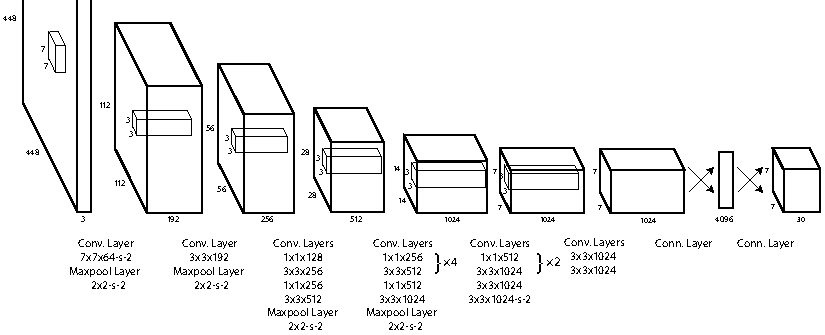
\includegraphics[width=0.90\linewidth]{rys_ok/Yolov1Struct.pdf} 
%            \caption{Struktura sieci Yolo \cite{yolov1}}
%\end{figure} 


\subsection{Yolo v2}
Detektor obiektów YOLO v2 wykorzystuje jednoetapową sieć detekcji obiektów. YOLO v2 jest szybszy niż dwuetapowe detektory obiektów z głębokim uczeniem, takie jak regiony z sieciami neuronowymi splotowymi (Faster R-CNN). Model YOLO v2 uruchamia sieć neuronową głębokiego uczenia (CNN) na obrazie wejściowym w celu wygenerowania predykcji sieciowych. Detektor obiektów dekoduje predykcje i generuje pola ograniczające. \cite{yolov2Matlab}

Architektura Darknet-19. Aby przyspieszyć i zwiększyć wydajność modelu, YOLOv2 wprowadził nową architekturę o nazwie „Darknet 19”. Nazwa tej architektury pochodzi od 19 warstw splotowych. Dla porównania, oryginalny YOLOv1 miał 8,5 miliarda parametrów, podczas gdy Darknet 19 zredukował je do 5,5 miliarda. Darknet 19 jest nie tylko wydajny, ale i wydajny. Jeśli chodzi o klasyfikację obrazów, konkuruje z wiodącymi modelami, takimi jak VGG czy ResNet, zachowując jednocześnie wysoką prędkość 200 klatek na sekundę (FPS). Oryginalny YOLOv1 był już znany ze swojej szybkości i dokładności, a Darknet 19 bazuje na tym dziedzictwie. Modyfikacje wprowadzone w Darknecie 19 w zakresie wykrywania obiektów obejmują usunięcie ostatnich w pełni połączonych warstw i ostatecznej warstwy klasyfikacji. W ich miejsce dodano trzy warstwy splotowe, a następnie warstwę „przelotową”, o której mówiliśmy wcześniej. Ta warstwa przelotowa łączy mapy cech w określony sposób, tworząc ostateczną mapę cech o wymiarach 13x13x125, która służy do wykrywania obiektów \cite{yolov2medium}.

%\begin{figure}[ht]
%    	\centering 
%            \includegraphics[width=0.60\linewidth]{rys_ok/yolo2_sctuct1.jpg} 
%            \caption{Realizacja sieci Yolo2 struktura Darknet-19 \cite{yolov2medium}}
%\end{figure} 

%\begin{figure}[ht]
%    	\centering 
%            \includegraphics[width=0.95\linewidth]{rys_ok/Yolo2_struct2.jpg} 
%            \caption{Realizacja sieci Yolo2 struktura Darknet-19 \cite{yolov2medium}}
%\end{figure} 



\subsection{Yolo v3}
Detektor obiektów YOLO v3 to wieloskalowa sieć detekcji obiektów, która wykorzystuje sieć ekstrakcji cech i wiele głowic detekcyjnych do tworzenia prognoz w wielu skalach. Model detekcji obiektów YOLO v3 uruchamia na obrazie wejściowym splotową sieć neuronową (CNN) z głębokim uczeniem, aby generować prognozy sieciowe z wielu map cech. Detektor obiektów gromadzi i dekoduje prognozy, aby generować pola ograniczające. YOLO v3 do prognozowanie obiektów na obrazie w używa pól zakotwiczenia, przewiduje te trzy atrybuty dla każdego pola zakotwiczenia.
przecięcie przez sumę (IoU), przesunięcia pól zakotwiczenia i prawdopodobieństwo klasy - etykietę klasy przypisaną do każdego pola zakotwiczenia.  \cite{yolov3Matlab}

\begin{figure}[ht]
    	\centering 
            \includegraphics[width=0.8\linewidth]{rys_ok/yolo3_struct.jpg} 
            \caption{YOLO-V3 budowa \cite{yolov3Matlab}}
\end{figure} 

\begin{figure}[ht]
    	\centering 
            \includegraphics[width=0.8\linewidth]{rys_ok/yolo3arch.jpg} 
            \caption{YOLO-V3 struktura źródło: Uri Almog \cite{yolov3Uri}}
\end{figure} 


\subsection{Yolo v4}
Sieć detekcji obiektów YOLO v4 to jednoetapowa sieć detekcji obiektów, składająca się z trzech części: szkieletu (backbone), szyi (neck) i podstawy (head). Szkielet może być wstępnie wytrenowaną splotową siecią neuronową, taką jak VGG16 lub CSPDarkNet53, trenowaną na zbiorach danych COCO lub ImageNet. Szkielet sieci YOLO v4 pełni funkcję sieci ekstrakcji cech, która oblicza mapy cech z obrazów wejściowych.
Szyja (neck) łączy szkielet z podstawą. Składa się ona z modułu puli piramid przestrzennych (SPP) i sieci agregacji ścieżek (PAN). Szyja (neck) łączy mapy cech z różnych warstw sieci szkieletowej i przesyła je jako dane wejściowe do podstawy (head).
Podstawa (head) przetwarza zagregowane cechy i przewiduje pola ograniczające, wyniki obiektowości i wyniki klasyfikacji. Sieć YOLO v4 wykorzystuje jednoetapowe detektory obiektów, takie jak YOLO v3, jako głowice detekcyjne.
Moduł SPP w szyjce łączy dane wyjściowe funkcji max-pooling mapy cech o niskiej rozdzielczości w celu ekstrakcji najbardziej reprezentatywnych cech. Moduł SPP wykorzystuje jądra o rozmiarach 1x1, 5x5, 9x9 i 13x13 do operacji max-pooling. Wartość kroku jest ustawiona na 1. Łączenie map cech zwiększa pole odbioru cech szkieletu i zwiększa dokładność sieci w wykrywaniu małych obiektów. Połączone mapy cech z modułu SPP są łączone z mapami cech o wysokiej rozdzielczości za pomocą modułu PAN. Moduł PAN wykorzystuje operacje upsamplingu i downsamplingu do wyznaczania ścieżek od dołu do góry i od góry do dołu, łącząc cechy niskiego i wysokiego poziomu.
Moduł PAN generuje zestaw zagregowanych map cech do wykorzystania w predykcjach. Sieć YOLO v4 ma trzy głowice detekcyjne. Każda głowica detekcyjna to sieć YOLO v3, która oblicza ostateczne predykcje. Sieć YOLO v4 generuje mapy cech o rozmiarach 19x19, 38x38 i 76x76, aby przewidywać pola ograniczające, wyniki klasyfikacji i wyniki obiektowości.
Tiny YOLO v4 to lekka wersja sieci YOLO v4 z mniejszą liczbą warstw sieciowych. Tiny YOLO v4 wykorzystuje sieć piramidy cech jako szyję i ma dwie głowice detekcyjne YOLO v3. Wyjścia sieciowe zawierają mapy o rozmiarach 13x13 i 26x26, służące do obliczania prognoz.
\cite{yolov4Matlab}
\begin{figure}[ht]
    	\centering 
            \includegraphics[width=0.8\linewidth]{rys_ok/yolov4architecture.jpg} 
            \caption{YOLO-V4\cite{yolov4Matlab}}
\end{figure} 



\subsection{Yolo v5}
Ultralytics YOLOv5 to najnowocześniejszy, najnowocześniejszy (SOTA) model widzenia komputerowego opracowany przez Ultralytics . Oparty na frameworku PyTorch , YOLOv5 słynie z łatwości obsługi, szybkości i dokładności. Wykorzystuje on wnioski i najlepsze praktyki z szeroko zakrojonych badań i rozwoju, co czyni go popularnym wyborem do szerokiego zakresu zadań sztucznej inteligencji w zakresie widzenia, w tym wykrywania obiektów , segmentacji i klasyfikacji obrazów (https://docs.ultralytics.com/yolov5/)\cite{ultralytics_doc}.
Yolo w wersji 5 nie występuje natywnie dla Matlab.

\subsection{Meituan Yolo v6}
Meituan YOLOv6 to najnowocześniejszy detektor obiektów, który oferuje niezwykłą równowagę między szybkością a dokładnością, co czyni go popularnym wyborem w aplikacjach czasu rzeczywistego. Model ten wprowadza kilka istotnych ulepszeń w architekturze i schemacie treningowym, w tym implementację modułu konkatenacji dwukierunkowej (BiC), strategię treningu wspomaganego kotwicą (AAT) oraz ulepszoną konstrukcję szkieletu i szyi, zapewniającą najwyższą dokładność w zbiorze danych COCO. Diagram architektury modelu przedstawiający przeprojektowane komponenty sieciowe i strategie treningowe, które doprowadziły do znacznej poprawy wydajności. (a) Szyja YOLOv6 (pokazano N i S). Uwaga: w przypadku M/L, RepBlocks jest zastępowany przez CSPStackRep. (b) Struktura modułu BiC. (c) Blok SimCSPSPPF. Moduł konkatenacji dwukierunkowej (BiC): YOLOv6 wprowadza moduł BiC w szyjce detektora, wzmacniając sygnały lokalizacji i zapewniając wzrost wydajności przy pomijalnym spadku prędkości. Strategia treningu wspomaganego kotwicą (AAT): Ten model proponuje AAT korzystanie z zalet zarówno paradygmatów opartych na kotwicy, jak i bez kotwicy, bez obniżania wydajności wnioskowania. Ulepszona konstrukcja szkieletu i szyjki: Dzięki pogłębieniu YOLOv6 o kolejny etap w szkielecie i szyjce, model ten osiąga najnowocześniejszą wydajność w zbiorze danych COCO przy wejściu o wysokiej rozdzielczości.\cite{ultralytics_doc}.
\begin{figure}[ht]
    	\centering 
            \includegraphics[width=0.95\linewidth]{rys_ok/yolo6struct.jpg} 
            \caption{YOLO-V6\cite{ultralytics_doc}}
\end{figure} 
Yolo w wersji 6 nie występuje natywnie dla Matlab.


\subsection{Yolo v7}
YOLOv7 to najnowocześniejszy detektor obiektów w czasie rzeczywistym, który przewyższa wszystkie znane detektory obiektów zarówno szybkością, jak i dokładnością w zakresie od 5 do 160 klatek na sekundę. Ma najwyższą dokładność (56,8\% AP) spośród wszystkich znanych detektorów obiektów w czasie rzeczywistym z 30 klatkami na sekundę lub więcej na GPU V100. Co więcej, YOLOv7 przewyższa inne detektory obiektów, takie jak YOLOR, YOLOX, Scaled-YOLOv4, YOLOv5 i wiele innych pod względem szybkości i dokładności. Model jest trenowany od podstaw na zbiorze danych MS COCO, bez użycia innych zbiorów danych ani wstępnie wytrenowanych wag.  

Wykrywanie obiektów w czasie rzeczywistym jest ważnym elementem wielu systemów widzenia komputerowego, w tym śledzenia wielu obiektów, autonomicznej jazdy, robotyki i analizy obrazów medycznych. W ostatnich latach rozwój detekcji obiektów w czasie rzeczywistym koncentrował się na projektowaniu wydajnych architektur i zwiększaniu szybkości wnioskowania różnych procesorów (CPU), procesorów graficznych (GPU) i neuronowych jednostek przetwarzania (NPU). YOLOv7 obsługuje zarówno mobilne procesory graficzne (GPU), jak i urządzenia GPU, od krawędzi sieci po chmurę.
W przeciwieństwie do tradycyjnych detektorów obiektów w czasie rzeczywistym, które koncentrują się na optymalizacji architektury, YOLOv7 koncentruje się na optymalizacji procesu uczenia. Obejmuje to moduły i metody optymalizacji zaprojektowane w celu zwiększenia dokładności wykrywania obiektów bez zwiększania kosztów wnioskowania, co jest koncepcją znaną jako treningowy „worek-rzeczy”.

\subsection{Yolo v8}
YOLOv8 został wydany przez Ultralytics 10 stycznia 2023 roku, oferując najnowocześniejszą wydajność pod względem dokładności i szybkości. Opierając się na udoskonaleniach poprzednich wersji YOLO, YOLOv8 wprowadził nowe funkcje i optymalizacje, które czynią go idealnym wyborem do różnych zadań wykrywania obiektów w szerokim zakresie zastosowań\cite{ultralytics_doc}.
\begin{figure}[ht]
    	\centering 
            \includegraphics[width=0.5\linewidth]{rys_ok/yolo8.jpg} 
            \caption{YOLO V8\cite{yolov8ar}}
\end{figure} 

Implementacja Yolo8 dla Matlab
To repozytorium oferuje różnorodne, wstępnie wytrenowane sieci YOLO v8 do wykrywania obiektów i segmentacji instancji w MATLAB®. Sieci te są trenowane na zbiorze danych COCO 2017[2] i umożliwiają wykrywanie 80 różnych kategorii obiektów, w tym osób, samochodów, sygnalizacji świetlnej itp. Ponadto repozytorium obsługuje trenowanie niestandardowych detektorów obiektów w celu precyzyjnego dostrojenia modeli do konkretnych zastosowań.
Oprogramowanie i wagi modeli są udostępniane na licencji GNU Affero General Public License v3.0.\cite{yolov8Matlab} 

\subsection{Yolo v9}
YOLOv9 to znaczący postęp w dziedzinie wykrywania obiektów w czasie rzeczywistym, wprowadzając przełomowe techniki, takie jak programowalna informacja gradientowa (PGI) i uogólniona efektywna sieć agregacji warstw (GELAN). Model ten charakteryzuje się znaczną poprawą wydajności, dokładności i adaptacyjności, wyznaczając nowe standardy w zbiorze danych MS COCO. Projekt YOLOv9, choć rozwijany przez odrębny zespół open source, opiera się na solidnej bazie kodu dostarczonej przez Ultralytics YOLOv5, co świadczy o duchu współpracy społeczności badawczej zajmującej się sztuczną inteligencją.

\begin{figure}[ht]
    	\centering 
            \includegraphics[width=0.8\linewidth]{rys_ok/yolo9.jpg} 
            \caption{YOLO V9\cite{yolov9}}
\end{figure} 

Informacje o implementacji modelu Yolo v9 dla Matlab\cite{yolov9matlab}




\subsection{Yolo v10}
Yolo v10 oparty na pakiecie Ultralytics Python, opracowany przez naukowców z Uniwersytetu Tsinghua, wprowadza nowe podejście do wykrywania obiektów w czasie rzeczywistym, rozwiązując zarówno problemy związane z postprocessingiem, jak i architekturą modelu, które wystąpiły we wcześniejszych wersjach YOLO. Dzięki wyeliminowaniu tłumienia niemaksymalnego (NMS) i optymalizacji różnych komponentów modelu, YOLOv10 osiąga najwyższą wydajność przy znacznie zmniejszonym narzucie obliczeniowym. Obszerne eksperymenty wykazują korzystny kompromis między dokładnością a opóźnieniem w wielu skalach modelu. \cite{ultralytics_doc}

\begin{figure}[ht]
    	\centering 
            \includegraphics[width=0.8\linewidth]{rys_ok/yolo10.jpg} 
            \caption{YOLO V10\cite{ultralytics_doc}}
\end{figure} 
Yolo w wersji 6 nie występuje natywnie dla Matlab.

\subsection{Yolo v11}
YOLO11 to najnowsza wersja detektorów obiektów w czasie rzeczywistym z serii Ultralytics YOLO, która na nowo definiuje możliwości dzięki najnowocześniejszej dokładności, szybkości i wydajności. Opierając się na imponujących postępach poprzednich wersji YOLO, YOLO11 wprowadza znaczące ulepszenia w architekturze i metodach uczenia, czyniąc go wszechstronnym wyborem do szerokiego zakresu zadań z zakresu wizji komputerowej.YOLO11 wykorzystuje ulepszoną architekturę szkieletową i szyjową, która rozszerza możliwości ekstrakcji cech, zapewniając precyzyjniejsze wykrywanie obiektów i wydajność złożonych zadań. YOLO11 wprowadza udoskonalone projekty architektoniczne i zoptymalizowane procesy szkoleniowe, zapewniając większą prędkość przetwarzania i zachowując optymalną równowagę między dokładnością a wydajnością.
Większa dokładność przy mniejszej liczbie parametrów: Dzięki ulepszeniom w projektowaniu modeli, YOLO11m osiąga wyższą średnią precyzję (mAP) w zbiorze danych COCO, wykorzystując o 22\% mniej parametrów niż YOLOv8m, co zapewnia wydajność obliczeniową bez utraty dokładności.YOLO11 można bezproblemowo wdrożyć w różnych środowiskach, w tym na urządzeniach brzegowych, platformach chmurowych i systemach obsługujących procesory graficzne NVIDIA, co zapewnia maksymalną elastyczność. Szeroki zakres obsługiwanych zadań: Niezależnie od tego, czy chodzi o wykrywanie obiektów, segmentację instancji, klasyfikację obrazów, estymację pozycji, czy zorientowane wykrywanie obiektów (OBB), YOLO11 został zaprojektowany z myślą o zróżnicowanym zestawie wyzwań związanych z przetwarzaniem obrazu.\cite{yolov11}

\begin{figure}[ht]
    	\centering 
            \includegraphics[width=0.4\linewidth]{rys_ok/yolo11.jpg} 
            \caption{YOLO V10\cite{yolov11medium}}
\end{figure} 
Yolo w wersji 11 nie występuje natywnie dla Matlab.


\subsection{Yolo 12}
Architekturę skoncentrowaną na uwadze, która odchodzi od tradycyjnych podejść opartych na sieciach neuronowych (CNN) stosowanych w poprzednich modelach YOLO, zachowując jednocześnie szybkość wnioskowania w czasie rzeczywistym, niezbędną w wielu zastosowaniach. Model ten osiąga najnowocześniejszą dokładność wykrywania obiektów dzięki nowatorskim innowacjom metodologicznym w mechanizmach uwagi i ogólnej architekturze sieci, zachowując jednocześnie wydajność w czasie rzeczywistym.
Mechanizm uwagi obszarowej: Nowe podejście do samouważności, które efektywnie przetwarza duże pola recepcyjne. Dzieli mapy obiektów na l obszarów o równej wielkości (domyślnie 4), poziomo lub pionowo, unikając skomplikowanych operacji i utrzymując duże efektywne pole recepcyjne. To znacznie zmniejsza koszty obliczeniowe w porównaniu ze standardową samouważnością.[...]
Implementacja Ultralytics YOLO12 domyślnie nie wymaga FlashAttention. FlashAttention można jednak opcjonalnie skompilować i używać z YOLO12. Do kompilacji FlashAttention potrzebny jest jeden z następujących procesorów graficznych NVIDIA:
\begin{itemize}
    \item GPU Turing (np. seria T4, Quadro RTX)
    \item GPU Ampere (np. seria RTX30, A30/40/100)
    \item GPU Ada Lovelace (np. seria RTX40)
    \item GPU Hopper (np. H100/H200) \cite{ultralytics_doc}.
\end{itemize}

\begin{figure}[ht]
    	\centering 
            \includegraphics[width=0.9\linewidth]{rys_ok/yolov12_vs_prev.png} 
            \caption{YOLO wersje wcześniejsza a wersja 12\cite{yolov12}}
\end{figure} 


\section{Wdrożenie Yolo w Matlab}

Uruchomienie modeli Yolo w wersjach oraz 2, 3, 4 oraz 8 dostępne jest poprzez instalację odpowiednich rozszerzeń. \cite{yolov2Matlab} \cite{yolov3Matlab} \cite{yolov4Matlab} \cite{yolov8Matlab}.

Zdjęcia użyte w kodzie pochodzą z 
\cite{imagedog},
\cite{imagedog2}



%https://www.mathworks.com/matlabcentral/fileexchange/179569-object-detection-and-instance-segmentation-using-yolo-v8?s_tid=srchtitle_support_results_1_yolo+v8
%v8:
% Load YOLO v8 model
%det = yolov8ObjectDetector('yolov8s');

% Analyze loaded model
%analyzeNetwork(det.Network);